\subsection{Glyph: \glyph{Macromolecule activity}}
\label{sec:af:macromolecule}

The \emph{macromolecule activity} is defined, as the name implies, as the activities of macromolecules, which are biochemical substances that are built up from the covalent linking of pseudo-identical units. Examples of macromolecules include proteins, nucleic acids (RNA, DNA), and polysaccharides (glycogen, cellulose, starch, etc.). Attempting to define a separate glyph for the activities of each of these different molecules would lead to an explosion of symbols in SBGN, so instead, \SBGNAFLone defines only one glyph for activity of all macromolecules. The same glyph is to be used for activity of a protein or peptide, a nucleic acid, a complex sugar, and so on. The exact nature of a particular macromolecule that the activity is coming from in a diagram is then clarified using its label and annotation. (Future levels of SBGN may subclass the macromolecule and introduce different glyphs to differentiate macromolecules.)

\begin{glyphDescription}

\glyphSboTerm SBO:

\glyphContainer A \glyph{macromolecule activity} is represented by a rectangular container with rounded corners, as illustrated in \fig{af:macromolecule}.

\glyphLabel A \glyph{macromolecule} is identified by a label placed in an unbordered box containing a string of characters.  The characters can be distributed on several lines to improve readability, although this is not mandatory.  The label box must be attached to the center of the container.  The label may spill outside of the container.

A \glyph{macromolecule} can also carry one or several \glyph{units of information} (\sect{af:unitInfo}). The units of information can characterize a domain, such as a binding site.  Particular \glyph{units of information} are available for describing the material type (\sect{af:material-types-cv}) and the conceptual type (\sect{af:conceptual-types-cv}) of a macromolecule.

\end{glyphDescription}

\begin{figure}[H]
  \centering
  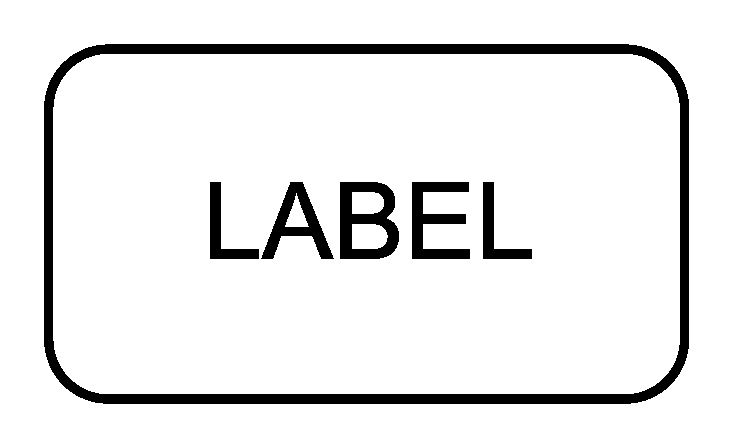
\includegraphics[width = 1.25in]{images/macromolecule-plain}
  \caption{The \AF glyph for \glyph{macromolecule activity}.}
  \label{fig:af:macromolecule}
\end{figure}
